\chapter{Implementierte Funktion zur Berechnung der Kreuz-Korrelation}
\label{chp:crosscorrelation:implementation}
Die Skripte zur Berechnung der Kreuz-Korrelation befinden sich im \enquote{crosscorrelation}-Verzeichnis.
Diese Skripte werden von den automatisierten Skripten verwendet.
Ein Aufrufen des hier beschriebenen Codes ist nur notwendig, wenn man eigene Skripte verfasst oder nur eine einzelne Funktion nutzen will.
Das Python Skript \enquote{functions\_crosscorrelation.py} bietet als Einstiegspunkt die Funktion\\ \mbox{\enquote{crossCorrelation(...)}} an. Im Folgenden werden die Parameter und deren Bedeutung beschrieben.
Im Anschluss werden die Auswirkungen der Parameter dargestellt.

\section{Beschreibung der Parameter}

Es gibt drei Parameter, die beim Aufruf der Funktion mitgegeben werden müssen. Dabei handelt es sich um die beiden Sequenzen, die verarbeitet werden sollen sowie um die Einstellungen. Aufgrund der vielen Einstellungsmöglichkeiten, wurden diese in eine eigene Klasse ausgelagert, die beim Aufruf als dritter Parameter übergeben werden muss.
\begin{description}[style=nextline]
\item[seqA] Die erste Datensequenz in Form eines eindimensionalen Arrays. Die enthaltenen Zahlenwerte müssen in Float konvertierbar sein.
\item[seqB] Die zweite Datensequenz in Form eines eindimensionalen Arrays. Die enthaltenen Zahlenwerte müssen in Float konvertierbar sein.
\item[settings] Die Einstellungen die verwendet werden sollen. 
\end{description}

\subsection{Einstellungsparameter}
Folgende Parameter stehen für die Konfiguration zur Verfügung. Die standardmäßig gesetzten Werte sind mit angegeben:
\begin{description}[style=nextline]
\item[plotNormalizedData] [Default: False] Auf True setzen, wenn die beiden Sequenzen auch normalisiert dargestellt werden sollen.
\item[plotCorrelations] [Default: False] Auf True setzen, wenn die berechnete Kreuz-Korrelation dargestellt werden soll. Dabei werden alle drei Berechnungsmethoden \enquote{Valid}, \enquote{Same} und \enquote{Full} dargestellt.
\item[plotNonNormalizedResults] [Default: False] Auf True setzen, wenn auch die unnormalisierten Ergebnisse dargestellt werden sollen.
\item[plotNormalizedResults] [Default: True] Auf False setzen, wenn auch die normalisierten Ergebnisse nicht dargestellt werden sollen.
\item[subtractMeanFromResult] [Default: True] Auf False setzen, wenn das arithmethische Mittel nicht von den Ergebnissen abgezogen werden soll.
\item[drawResults] [Default: False] Wird dieser Parameter auf True gesetzt, werden die Ergebnisse auf dem Bildschirm ausgegeben. Dies kann sinnvoll sein, wenn keine PDF-Dateien erstellt werden sollen, die Ergebnisse aber dennoch sichtbar sein sollten. Der Standardwert ist auf False gesetzt, da die Skripte automatisiert durch weitere Skripte aufgerufen werden. Die Verarbeitung der Skripte blockiert dabei solange das Fenster zur Anzeige geöffnet ist. In einem automatisierten Kontext würde niemand das Fenster schließen, wodurch der Prozess blockiert werden würde.
\item[exportToPdf] [Default: False] Auf True setzen, wenn eine PDF-Datei mit den Ergebnissen generiert werden soll.
\item[exportFilePath] [Default: \enquote{}] Der Pfad zur PDF-Datei, in dem die Ergebnisse gespeichert werden sollen. Wenn \enquote{exportToPdf} auf True gesetzt wird, muss mit dieser Einstellung der Pfad zur PDF-Datei angegeben werden. Ansonsten wird die Einstellung ignoriert.
\end{description}

\section{Beispiel Ergebnisse}
Es gilt für alle Beispiele (solange nicht im Beispiel genauer spezifiziert):\\
Vorbedingung: Zwei Sequenzen mit je 10000 Einträgen. \\
SeqA:
\[ a_{n} =
  \begin{cases}
    1       & \quad \text{wenn } n \text{ enthalten in [1005,2005,1505,3505,5505,6005,6505,8005,8505,9005]}\\
    0  & \quad \text{sonst}
  \end{cases}
\]
SeqB:
\[ b_{n} =
  \begin{cases}
    1       & \quad \text{wenn } n \text{ enthalten in [1000,2000,1500,3500,5500,6000,6500,8000,8500,9000]}\\
    0  & \quad \text{sonst}
  \end{cases}
\]
Es ist ersichlich, dass die Sequenzen zueinander um einen Index von 5 verschoben sind.

\subsection{Anzeige der beiden Sequenzen mit normalisiertem Ergebnis}
Der Aufruf der Funktion mit den Standard-Parametern der Einstellungen, liefert für die Beispielsequenzen folgendes Ergebnis (dargestellt in Abbildung~\ref{fig:correlationDefaultParams}):
\begin{figure}[H]
    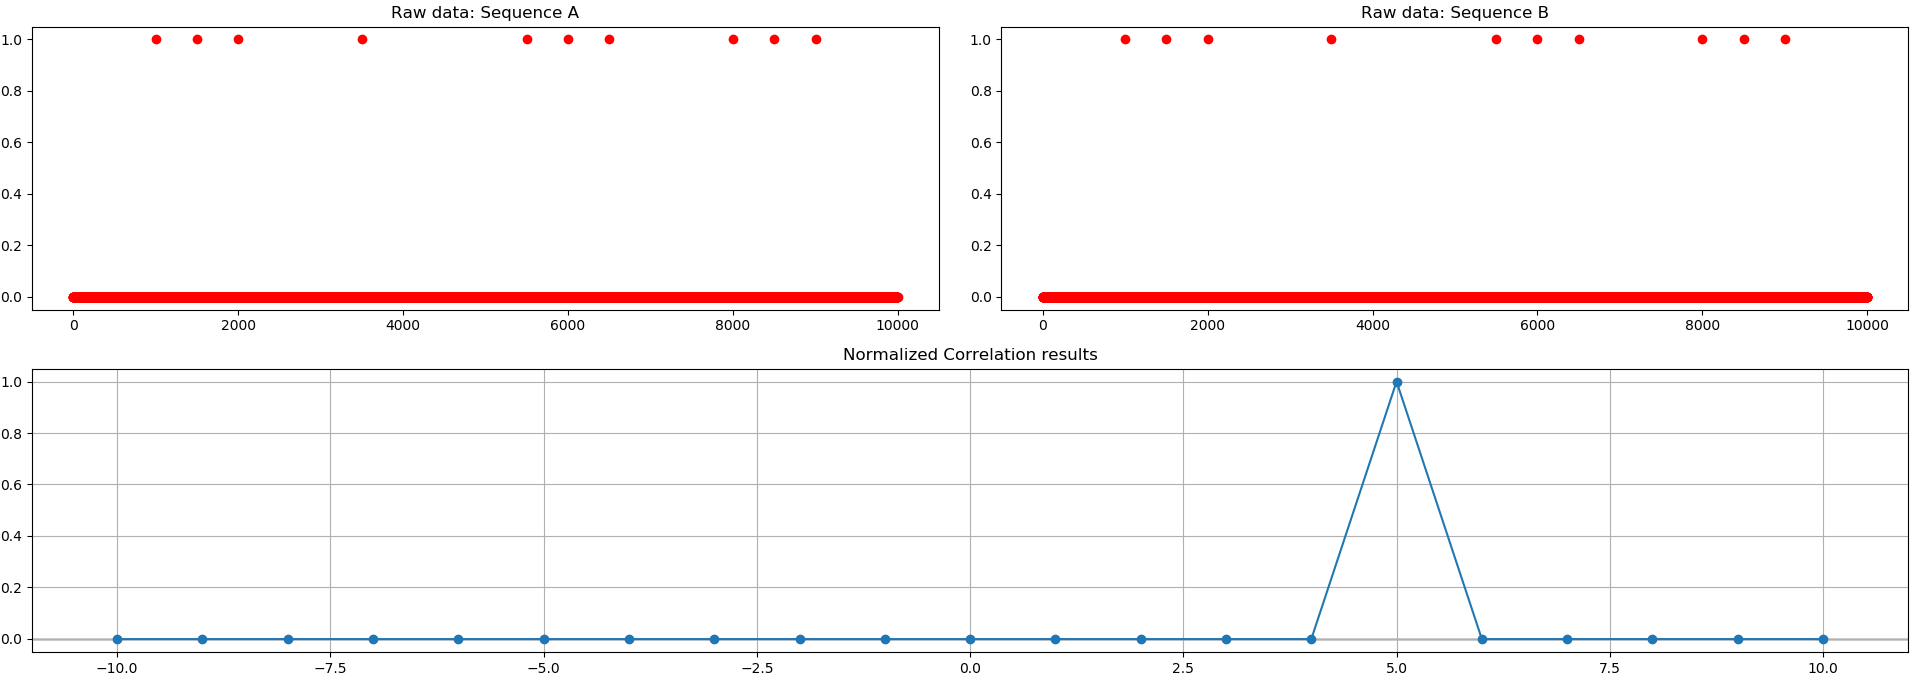
\includegraphics[width=\linewidth]{pythonImplementation/images/correlationDefaultParams.PNG}
    \caption[Ergebnis: Default-Parameter]{Ergebnis der Funktion bei Default-Parametern\footnotemark.}
    \label{fig:correlationDefaultParams}
\end{figure}
\footnotetext{ Quelle: Eigene Darstellung}

\subsection{Auswirkungen des Parameter: plotNormalizedData}
Durch Setzen des optionalen Parameters \enquote{plotNormalizedData} auf True, werden die beiden Sequenzen, zusätzlich in normalisierter Form dargestellt. 
Siehe dazu Abbildung~\ref{fig:correlationPlotNormalizedData}. 
\begin{figure}[H]
    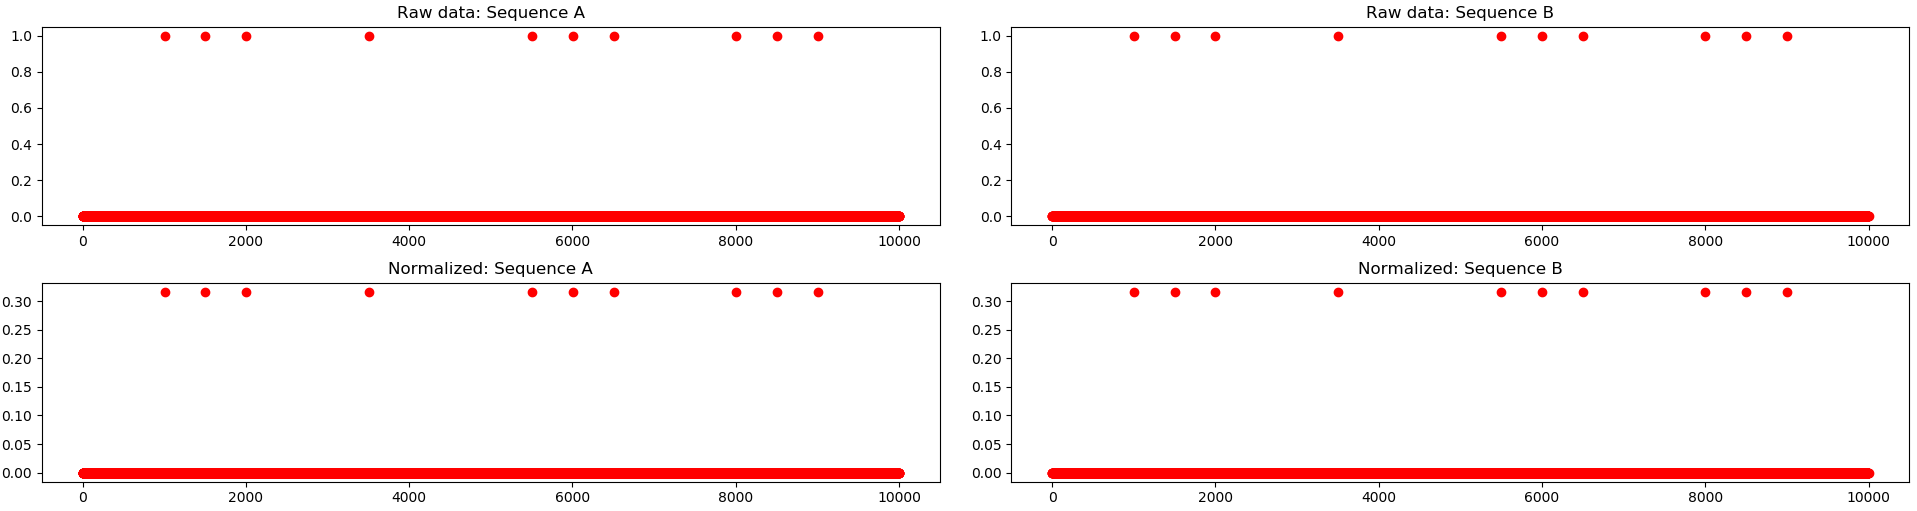
\includegraphics[width=\linewidth]{pythonImplementation/images/correlationPlotNormalizedData.PNG}
    \caption[Ergebnis: plotNormalizedData]{Ergebnis der Funktion bei \enquote{plotNormalizedData = True} (Darstellung der Ergebnisse weggelassen)\footnotemark. }
    \label{fig:correlationPlotNormalizedData}
\end{figure}
\footnotetext{ Quelle: Eigene Darstellung}

\subsection{Auswirkungen des Parameter: plotCorrelations}
Durch Setzen des optionalen Parameters \enquote{plotCorrelations} auf True, 
wird die Kreuz-Korrelation der beiden Sequenzen berechnet.
Dabei werden alle drei Berechnungsmethoden \enquote{Valid}, \enquote{Same} und \enquote{Full} dargestellt.
Siehe dazu Abbildung~\ref{fig:correlationPlotCorrelations}. 
\begin{figure}[H]
    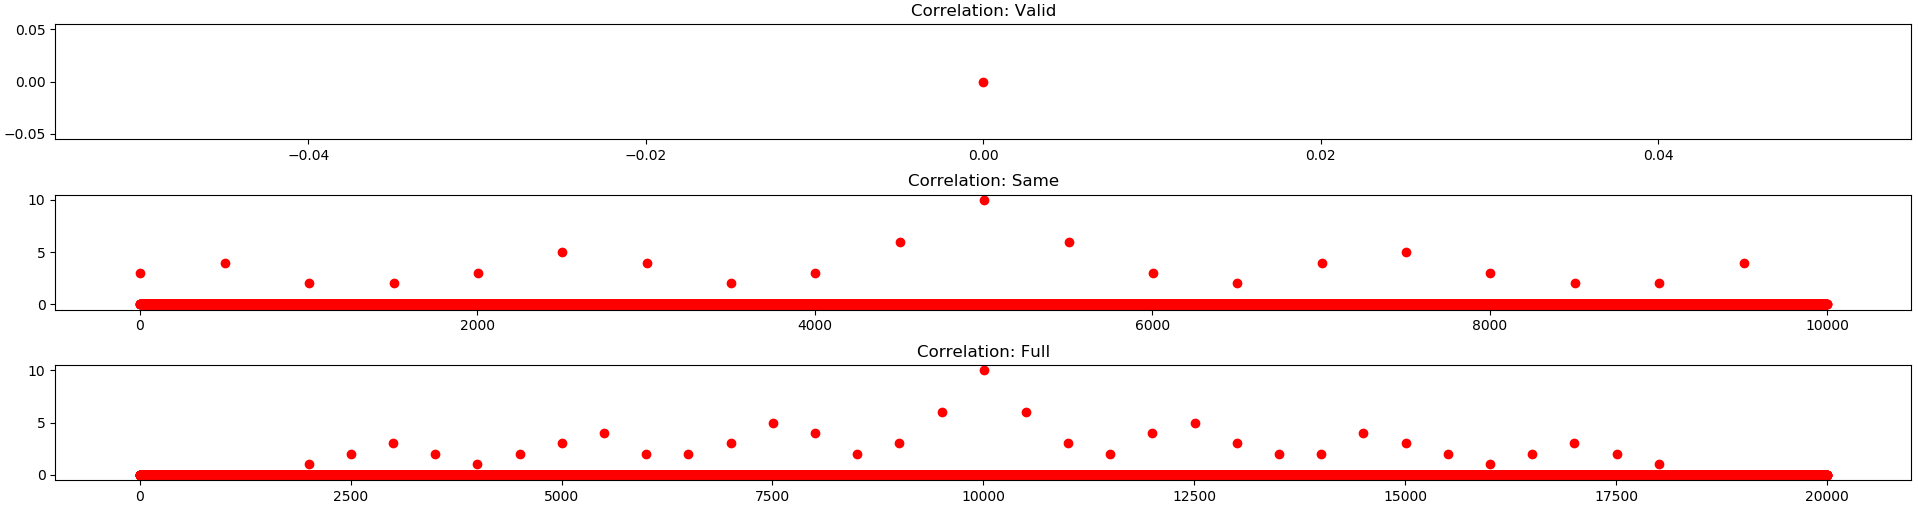
\includegraphics[width=\linewidth]{pythonImplementation/images/correlationPlotCorrelations.PNG}
    \caption[Ergebnis: plotCorrelations]{Zusätzliche Ausgabe der Funktion bei \enquote{plotCorrelations = True} (Darstellung der Ergebnisse weggelassen)\footnotemark. }
    \label{fig:correlationPlotCorrelations}
\end{figure}
\footnotetext{ Quelle: Eigene Darstellung}

\subsection{Auswirkungen des Parameter: plotNonNormalizedResults}
Durch Setzen des optionalen Parameters \enquote{plotNonNormalizedResults} auf True, können die Ergebnisse zusätzlich in unnormalisierter Form ausgegeben werden.
Siehe dazu Abbildung~\ref{fig:correlationPlotNonNormalizedResults}. 
\begin{figure}[H]
    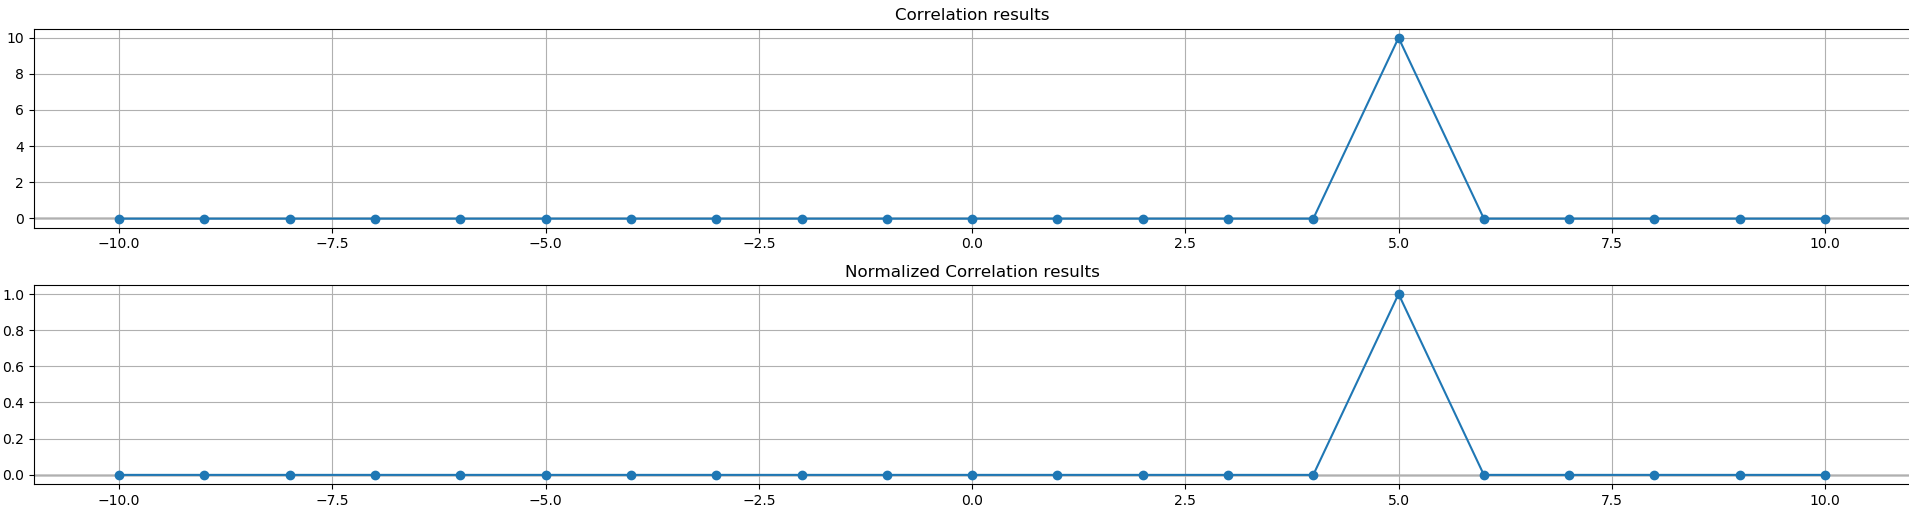
\includegraphics[width=\linewidth]{pythonImplementation/images/correlationPlotNonNormalizedResults.PNG}
    \caption[Ergebnis: plotNonNormalizedResults]{Zusätzliche Ausgabe der Funktion bei \enquote{plotNonNormalizedResults = True}\footnotemark. }
    \label{fig:correlationPlotNonNormalizedResults}
\end{figure}
\footnotetext{ Quelle: Eigene Darstellung}

\subsection{Auswirkungen des Parameter: plotNormalizedResults}
Durch Setzen des optionalen Parameters \enquote{plotNormalizedResults} auf False, kann die Ausgabe der normalisierten Ergebnisse verhindert werden.

\subsection{Auswirkungen des Parameter: subtractMeanFromResult}
Um die Auswirkung des Parameters darzustellen, werden folgende Sequenzen vorrausgesetzt (je 10000 Einträge):\\
SeqA:
\[ a_{n} =
  \begin{cases}
    2       & \quad \text{wenn } n \text{ enthalten in [1005,2005,1505,3505,5505,6005,6505,8005,8505,9005]}\\
    1  & \quad \text{sonst}
  \end{cases}
\]
SeqB:
\[ b_{n} =
  \begin{cases}
    2       & \quad \text{wenn } n \text{ enthalten in [1000,2000,1500,3500,5500,6000,6500,8000,8500,9000]}\\
    1  & \quad \text{sonst}
  \end{cases}
\]
Die Sequenzen sind wieder um einen Wert von 5 verschoben, allerdings wechseln diese nicht zwischen 0 und 1, sondern zwischen 1 und 2. 
Die Ergebnisse können dabei unübersichtlich werden, deshalb wird ohne Angabe des Parameters, True als Standardwert verwendet.
Dadurch wird das arithmethische Mittel des Ergebnis vom Ergebnis selbst abgezogen. Abbildung~\ref{fig:correlationSubtractMeamFromResultTrue} 
und \ref{fig:correlationSubtractMeamFromResultFalse} zeigen die Auswirkung des Parameters. 
\begin{figure}[H]
    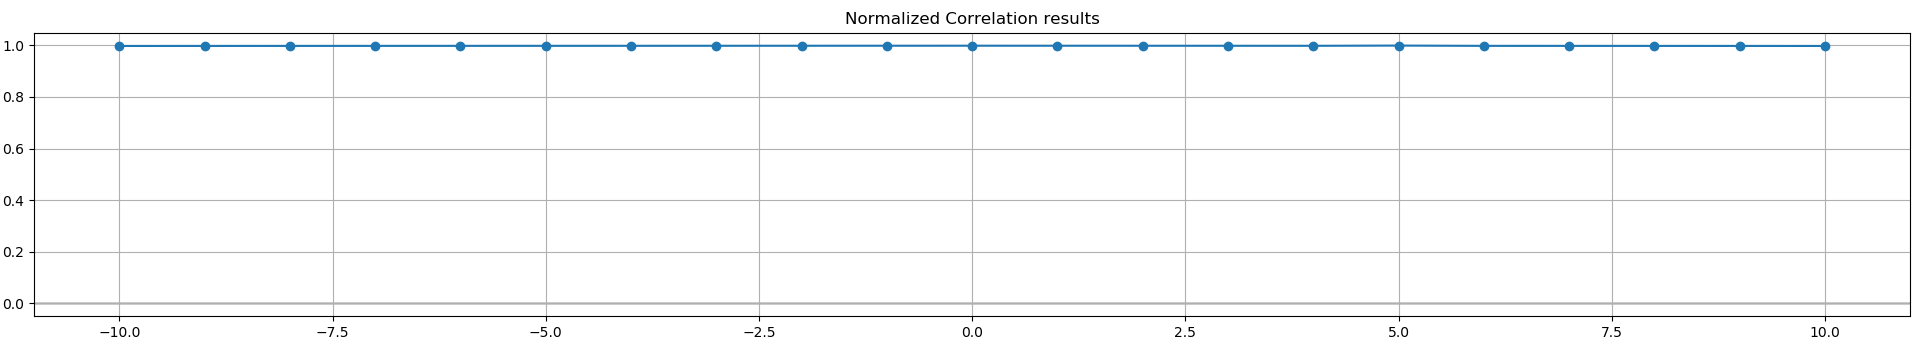
\includegraphics[width=\linewidth]{pythonImplementation/images/correlationSubtractMeamFromResultFalse.PNG}
    \caption[Ergebnis: subtractMeanFromResult = False]{Darstellung des Ergebnis bei \enquote{subtractMeanFromResult = False}. Ausschläge sind sehr schwer erkennbar\footnotemark. }
    \label{fig:correlationSubtractMeamFromResultFalse}
\end{figure}
\footnotetext{ Quelle: Eigene Darstellung}

\begin{figure}[H]
    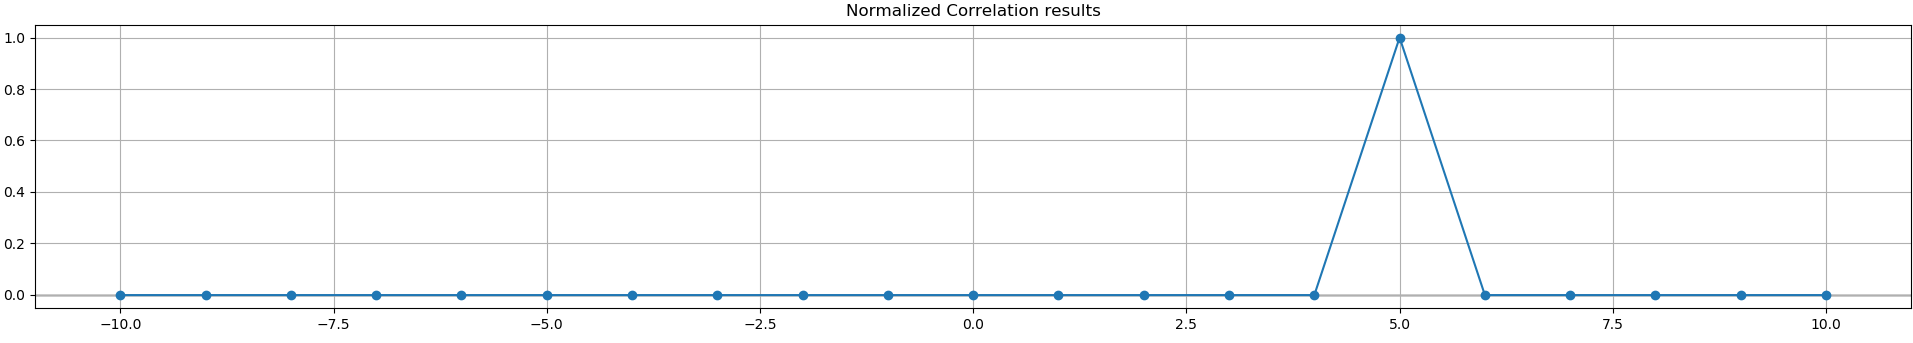
\includegraphics[width=\linewidth]{pythonImplementation/images/correlationSubtractMeamFromResultTrue.PNG}
    \caption[Ergebnis: subtractMeanFromResult = True]{Darstellung des Ergebnis bei \enquote{subtractMeanFromResult = True}. Ausschläge sind besser erkennbar\footnotemark. }
    \label{fig:correlationSubtractMeamFromResultTrue}
\end{figure}
\footnotetext{ Quelle: Eigene Darstellung}


\section{Beispiel-Skripte}
Ein Skript welches die Funktion aus diesem Kapitel nutzt ist als Beispiel im Projekt unter \enquote{example\_script\_crosscorrelation.py} abgelegt.\\
Das Skript das im Zuge der Automatisierung verwendet wird, ist im Unterverzeichnis \enquote{crosscorrelation} unter \enquote{automated\_crosscorrelation.py} zu finden.









\chapter{Suche nach Pattern mit Hilfe der Kreuz-Korrelation}
\label{chp:crosscorrelation:patternsearch}
Das Python Skript \enquote{functions\_crosscorrelation\_patternsearch.py} bietet zwei Funktionen an, die verwendet werden können, 
um nach einem gegebenen Pattern in einer Sequenz zu suchen.
Ein Beispiel für die Verwendung ist in \enquote{example\_script\_crosscorrelation.py} abgebildet.

\section{Angebotene Funktionen}
Folgende Funktionen werden angeboten:

\subsection{Funktion: getCorrelationDataForPatternSearch}
Mit Hilfe der \enquote{getCorrelationDataForPatternSearch} Funktion kann nach einem Pattern in einer gegebenen Sequenz gesucht werden. Dafür sind folgende Parameter nutzbar:
\begin{description}
    \item[seqA] Die Sequenz in der nach dem Pattern gesucht werden soll. Übergeben in Form eines eindimensionalen Arrays. Die enthaltenen Zahlenwerte müssen in Float konvertierbar sein.
    \item[pattern] Das Pattern nach dem gesucht werden soll. Übergeben in Form eines eindimensionalen Arrays. Die enthaltenen Zahlenwerte müssen in Float konvertierbar sein.
    \item[plotCorrelation] [Default: False] Auf True setzen, wenn die berechnete Kreuz-Korrelation auf dem Monitor dargestellt werden soll.
\end{description}
Die Funktion gibt die berechnete Kreuz-Korrelation zurück, die in der nächsten Funktion \enquote{extractIndicesFromCorrelationData} verwendet werden kann.
\\
\\
Die Funktion verwendet intern die von NumPy bereitgestellte \enquote{correlate} Funktion. Als Modus wird der in Kapitel~\ref{sec:numpy_correlate_mode} beschriebene Modus \enquote{Valid} genutzt.

\subsection{Funktion: extractIndicesFromCorrelationData}
Die Funktion kann verwendet werden, um die Indizes zu berechnen, an denen das Pattern in der Sequenz auftritt. Dafür muss der Funktion das Ergebnis der \enquote{getCorrelationDataForPatternSearch} Funktion
übergeben werden. Als Rückgabe erhält man die Indizes und der Wert der Korrelation an dieser Stelle.\\
Optional kann ein Schwellwert übergeben werden. Je nachdem wie dieser Schwellwert gewählt ist, werden mehr oder weniger Indizes zurückgegeben. Bei einem hohen Schwellwert wird 
jeweils nur der erste Index zurückgegeben, bei dem das Pattern auftritt. Bei einem niedriger gewählten Schwellwert werden alle Indizes zurückgegeben, an denen das Pattern auftritt. 
Bei einem zu niedrigem Schwellwert werden auch Indizes zurückgegeben, die außerhalb des eigentlichen Patterns liegen. Diese Bereiche befinden sich direkt vor und nach dem Ende des Patterns. Ein zu niedriger Schwellwert kann erkannt werden, wenn der gefundene Bereich größer als das Pattern selbst ist. Durch einen höheren Schwellwert kann dieses \enquote{Auswaschen} oder \enquote{Aufweichen} verhindert werden.

\subsection{Beispiel für die Pattern-Suche}
Vorbedingung: Eine Sequenz mit 10000 Einträgen. \\
SeqA:
\[ a_{n} =
  \begin{cases}
    1       & \quad \text{wenn } n \text{ enthalten in [1005,1007,1010,6005,6007,6010]}\\
    0  & \quad \text{sonst}
  \end{cases}
\]
Gesuchtes Pattern:
\[
pattern = [1,0,1,0,0,1,0] 
\]
Das Pattern tritt in der gegeben Sequenz zwei Mal auf (an Index 1005 und 6005).
Der Aufruf der \enquote{getCorrelationDataForPatternSearch} Funktion mit dem \enquote{plotCorellation = True} zeigt die in Abbildung~\ref{fig:patternsearchCorrelation} dargestellte Kreuz-Korrelation.

\begin{figure}[H]
  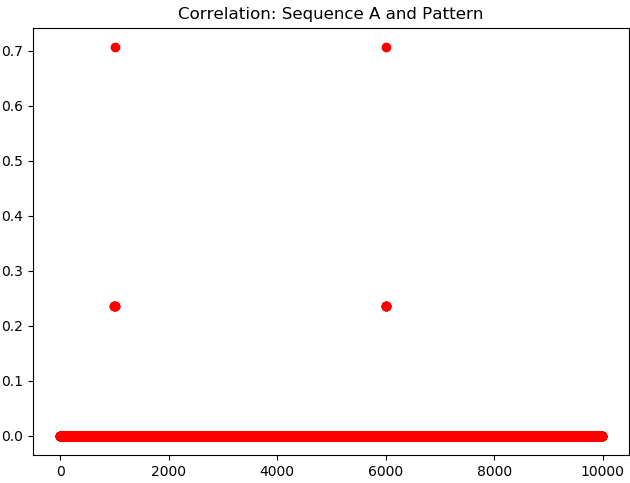
\includegraphics[width=\linewidth]{./images/patternsearchCorrelation.PNG}
  \caption[Patternsuche: Kreuz-Korrelation]{Kreuz-Korrelation der Patternsuche\footnotemark.}
  \label{fig:patternsearchCorrelation}
\end{figure}
\footnotetext{ Quelle: Eigene Darstellung}

\begin{samepage}
Mit Hilfe der dargestellten Kreuz-Korrelation kann der Schwellwert für die \enquote{extractIndicesFromCorrelationData} festgelegt werden.
Ein Aufruf mit einem Schwellwert von \enquote{0.3} liefert folgendes Ergebnis: \\
\begin{align*}
   & [6005, 0.70710678], \\
   & [1005, 0.70710678]
\end{align*}

Dabei handelt es sich um die Indizes, an denen das Pattern in der Sequenz beginnt (inklusive den Wert an dieser Stelle). \\
\end{samepage}
\begin{samepage}
Ein Aufruf mit einem Schwellwert von \enquote{0.2} liefert dagegen folgendes Ergebnis: \\
\begin{align*}
  &  [6005, 0.70710678], \\
  & [1005, 0.70710678], \\
  & [6003, 0.23570226], \\
  & [1000, 0.23570226], \\
  & [6007, 0.23570226], \\
  & [6010, 0.23570226], \\
  & [6002, 0.23570226], \\
  & [6000, 0.23570226], \\
  & [1010, 0.23570226], \\
  & [1008, 0.23570226], \\
  & [1007, 0.23570226], \\
  & [1003, 0.23570226], \\
  & [1002, 0.23570226], \\
 & [6008, 0.23570226]
\end{align*}
Darin enthalten sind Indizes im Bereich von 1000 bis 1010 sowie 6000 bis 6010. Die Bereiche sind größer als das Pattern selbst, allerdings ist das Pattern in diesen Bereichen enthalten.
\end{samepage}